\documentclass[a4paper,14pt]{extarticle} %размер бумаги устанавливаем А4, шрифт 14пунктов
\usepackage[T2A]{fontenc}
\usepackage[utf8]{inputenc}%включаем свою кодировку: koi8-r или utf8 в UNIX, cp1251 в Windows
\usepackage[english,russian]{babel}%используем русский и английский языки с переносами
\usepackage{amssymb,amsfonts,amsmath,mathtext,cite,enumerate,float} %подключаем нужные пакеты расширений

\usepackage{alltt}
\usepackage{fancyvrb}
%шрифт Times New Roman
%\usepackage{fontspec}
%\setmainfont{Times New Roman}
%\setallmainfonts{Times New Roman}

\usepackage{titlesec}

\makeatletter
\renewcommand{\@biblabel}[1]{#1.} % Заменяем библиографию с квадратных скобок на точку:
\makeatother

\usepackage{geometry} % Меняем поля страницы
\geometry{left=3cm}% левое поле
\geometry{right=15mm}% правое поле
\geometry{top=2cm}% верхнее поле
\geometry{bottom=2cm}% нижнее поле
\linespread{1.5}

\usepackage{indentfirst} % отделять первую строку раздела абзацным отступом
\setlength\parindent{5ex}
\setlength\parskip{-1em}
\usepackage{tikz}
\usepackage{pgfplots}
%links
\usepackage{url}

\usepackage[tableposition=top,singlelinecheck=false, justification=centering]{caption}
\usepackage{subcaption}

\usepackage{graphicx}
\graphicspath{{./pics/}}
\DeclareGraphicsExtensions{.pdf,.png,.jpg}

% маркированные списки
\renewcommand{\labelitemi}{-}
\renewcommand{\labelitemii}{-}
% нумерованные списки
\renewcommand{\labelenumi}{\asbuk{enumi})}
\renewcommand{\labelenumii}{\arabic{enumii})}

% номер сноски со скобкой
\renewcommand*{\thefootnote}{\arabic{footnote})}
\renewcommand{\footnoterule}{%
\kern -3pt
\hrule width 40mm height .4pt
\kern 2.6pt
}

%иллюстрации и таблицы
\DeclareCaptionLabelFormat{gostfigure}{Рис.#2}
\DeclareCaptionLabelFormat{gosttable}{Табл.#2}
\DeclareCaptionLabelSeparator{gost}{:~}
\captionsetup{labelsep=gost}
\captionsetup*[figure]{labelformat=gostfigure}
\captionsetup*[table]{labelformat=gosttable}
\renewcommand{\thesubfigure}{\asbuk{subfigure}}

\usepackage{tocloft}
\renewcommand{\cftsecleader}{\cftdotfill{\cftdotsep}}
%\renewcommand{\cfttoctitlefont}{\Large\filcenter}
%\setcounter{page}{3} %нумерация страниц с 3

\usepackage{listings}
\lstset{
frame=single,
breaklines=true
}

\usepackage{hyperref}
\hypersetup{
    colorlinks=true,
    linkcolor=blue,
    filecolor=magenta,      
    urlcolor=cyan,
    pdftitle={Overleaf Example},
    pdfpagemode=FullScreen,
    }

\author{Фоменко П.Г.}
\title{Электронная ведомость}

\begin{document}

\begin{flushright}
П.Г.Фоменко\\
5823
\end{flushright}

\section{Демозайкинг}

\subsection{Задание}
Получить .raw- файлы, выполнить процедуру демозайкинга(или интерполяции).\\

\subsection{Сложности, возникшие в ходе работы}
Алгоритм рассматривался на лекции, причём несколько разных, странно, что мы реализовывали лишь один. Очень наглядно он описан \href{https://medium.com/swlh/image-demosaicing-bilinear-interpolation-vs-high-quality-linear-interpolation-5fd2268c4c7a}{на этой странице} \\
Единственная не очевидная для меня вещь в этом задании была связана с представлением данных. А именно, хранение 12 бит информации в 2 байтах. Скорее всего, я просто не услышал этот момент из-за проблем с сетью.\\

\subsection{Предложение}
В статье на сайте Стэнфорда, посвящённой этому вопросу рассматриваются несколько различных алгоритмов, а затем сравнивается их эффективность с помощью PSNR. Возможно, в новой работе стоит сделать нечто подобное.\\
Сама статья: \href{https://stanford.edu/class/ee367/reading/Demosaicing_ICASSP04.pdf}{тут}.\\

\pagebreak

\section{Авто-баланс белого}

\subsection{Задание}
Для полученного после выполнения первого пункта изображения выполнить процедуру баланса белого с разными алгоритмами.\\

\subsection{Сложности, возникшие в ходе работы}
Основная сложность была связана с названием алгоритмов(путался сам и путал этим тех, у кого спрашивал об этом).\\

\subsection{Предложение}
Непосредственно в лабораторной работе можно будет сравнивать несколько различных алгоритмов баланса белого, может быть возможно как-нибудь численно выражать разницу между полученными изображениями(средний квадрат разности или коэффициент корреляции)?\\

\pagebreak

\section{Гамма-коррекция и эквализация гистограмм}

\subsection{Задание}
Для изображений, полученных в ходе выполнения второго задания выполнить гамма-коррекцию и эквализацю гистограмм. 

\subsection{Сложности, возникшие в ходе работы}
Материалов из лекций и книг, которые скидывали в дискорд-канал было достаточно для выполнения работы, а некоторые функции numpy заметно ускорили написание алгоритма эквализации гистограмм. Однако, в самом начале выполнения задания я забыл, что работать надо в другом цветовом пространстве и только с яркостной компонентой. 

\subsection{Предложение}
Добавить к этому заданию мне нечего. Гистограммы до и после эквализации, которые я забыл показать, представлены ниже.\\

\begin{figure}[H]
   \begin{minipage}{0.5\textwidth}
     \centering
     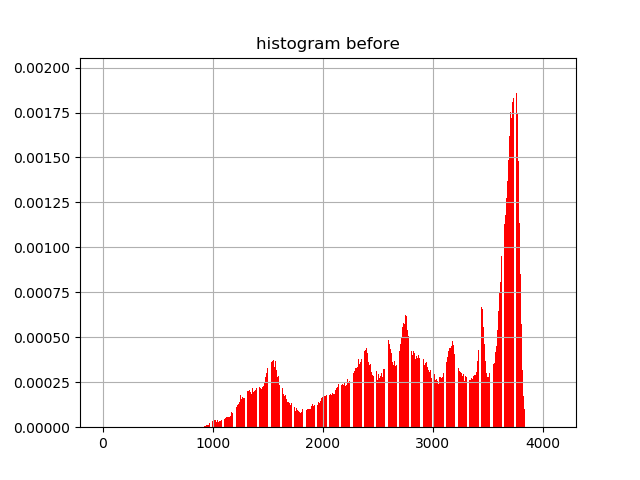
\includegraphics[width=\linewidth]{Figure_1}
     \caption{Гистограмма изображения до эквализации}\label{Fig:hist1}
   \end{minipage}\hfill
   \begin{minipage}{0.5\textwidth}
     \centering
     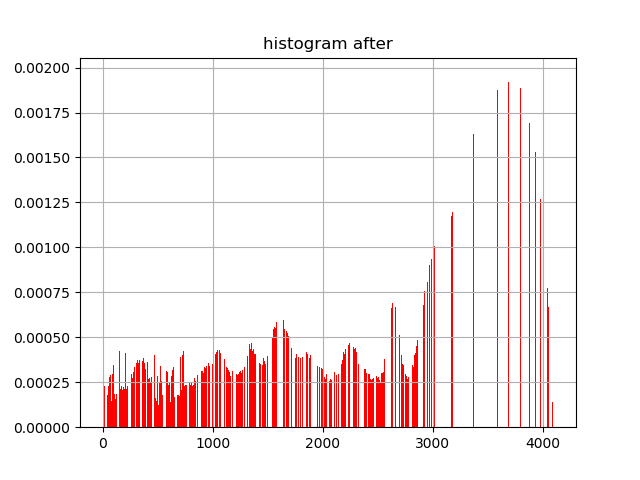
\includegraphics[width=\linewidth]{Figure_2}
     \caption{Гистограмма изображения после эквализации}\label{Fig:hist2}
   \end{minipage}
\end{figure}

\pagebreak

\section{Гауссовский и билатеральный фильтры}

\subsection{Задание}
Последняя часть ISP, применение к выровненным изображениям фильтры, для сглаживания(уменьшения уровня шума).
  
\subsection{Сложности, возникшие в ходе работы}
С Гауссовским фильтром проблем не возникло. Реализация билатерального фильтра "в лоб" \ не даёт хороших результатов по вычислительной эффективности.   

\subsection{Предложение}
Я бы хотел довести до конца реализацию билатерального фильтра, и если будет такая возможность помочь в его описании в методических указаниях к новой работе. 

\pagebreak


\end{document}








